\documentclass{article}

\usepackage{polski}
\usepackage[utf8]{inputenc}
\usepackage{booktabs}
\usepackage{graphicx}
\usepackage{float}
\usepackage{geometry}
\geometry{
	a4paper,
	total={170mm,257mm},
	left=35mm,
	right=35mm,
	top=35mm,
	bottom = 25mm
}


\begin{document}
	\newgeometry{tmargin=2cm, bmargin=2cm, lmargin=2cm, rmargin=2cm}
	
	\begin{titlepage}
		\center
		\newcommand{\HRule}{\rule{\linewidth}{0.5mm}}
		
		\textsc{\LARGE Politechnika Wrocławska}\\[1.5cm]
		\textsc{\Large Projekt}\\[0.5cm] 
		\textsc{\large Zarządzanie w systemach i sieciach komputerowych}\\[0.5cm] 

		\HRule \\[0.4cm]
		{ \huge \bfseries Analiza wpływu liczby procesów na czas działania algorytmów dla problemu komiwojażera}\\[0.4cm]
		\HRule \\[1.5cm]
		
		\begin{minipage}{0.4\textwidth}
			\begin{flushleft} \large
				\emph{Authors:}\\
				Rafał \textsc{Pieniążek} 
				\\ Jakub \textsc{Pomykała}
			\end{flushleft}
		\end{minipage}
		~
		\begin{minipage}{0.4\textwidth}
			\begin{flushright} \large
				\emph{Supervisor:} \\
				Dr inż. Robert \textsc{Wójcik} 
			\end{flushright}
		\end{minipage}\\[4cm]

		{\large \today}\\[3cm]
		
		\vfill
		
	\end{titlepage}

\tableofcontents
\newpage
	
	
	
	
\section{Wstęp}
	\subsection{Cel projektu}
	\subsection {Zakres projektu}
\section{Sformułowanie problemu}
		Problem komiwojażera jest problemem optymalizacyjnym, polegającym na znalezieniu ścieżki pomiędzy ustalonymi miastami dla następujących warunków: 
		\begin{itemize}
			\item wszystkie miasta są odwiedzone dokładnie jeden raz
			\item rozpoczynamy i kończymy w tym samym mieście.
			\item koszt (suma wag krawędzi) jest najmniejszy z wszystkich możliwych
		\end{itemize}
		Oznacza to, że należy znaleźć taki cykl Hamiltona dla grafu reprezentującego zbiór miast, dla którego suma wag wybranych krawędzi jest najmniejsza.
		
	\subsection{Opis wariantów problemu}	
		\subsubsection{Przegląd zupełny}
		\subsubsection{Branch\&Bound}
			
				W rozwiązaniu powyższego problemu zastosowano metodę podziału i ograniczeń. Metoda ta jest metodą optymalizacji dyskretnej, opierając się na podejściu \textit{dziel i zwycięzaj}.
				W każdym kroku algorytmu przeglądane jest drzewo potencjalnych rozwiązań. Jeżeli natrafimy na węzeł, który jest liściem, czyli można określić dla niego długość drogi komiwojażera,sprawdzamy, czy nowo znaleziona wartość nie jest lepsza od aktualnie zapisanej. Jeżeli tak jest, to zapamiętujemy nowe rozwiązanie. W przypadku, gdy dany węzeł nie jest liściem, tworzymy dla niego podproblemy. W tym celu odwiedzamy kolejne miasto starając się oszacować dolne ograniczenie kosztów całej trasy. W tym projekcie wykorzystano najprostszy sposób szacowania. Na początku z macierzy sąsiedztwa wycinana jest przekątna, następnie kolumny i wiersze miejsc już odwiedzonych. Następnie wartości z tak przygotowanej macierzy są sortowane w kolejności niemalejącej. Szacowanie polega na dodaniu do siebie tylu kolejnych wartości z listy, ile zostało miast do odwiedzenia. W niniejszym projekcie do przetrzymywania drzewa rozwiązań wykorzystano listę jednokierunkową. Wybór wynika z faktu, iż i tak należy przejrzeć wszystkie możliwe węzły, aby sprawdzić, czy ich ograniczenie nie jest większe niż aktualnie znalezione.
				
\section{Projekt aplikacji}	
	\subsection{Wybrane klasy}
	
		\subsubsection{Matrix}
		\subsubsection{Edge}
		\subsubsection{Node}
		
	\subsection{Realizacja algorytmów wyznaczania rozwiązań}
		\subsubsection{Przegląd zupełny}
		\subsubsection{Branch\&Bound}
		
	\subsection{Odczyt i zapis danych}
		\subsubsection{Wczytywanie z plików .tsp}	
		\subsubsection{Wczytywanie macierzy}
		\subsubsection{Generowanie danych losowych}
		\subsubsection{Generwoanie plikóW cvs}
\section{Testowanie wydajności}	
	\subsection{Czasy wykonania algorytmów}
		\subsubsection{Czas działania algorytmu metodą podziału i ograniczeń}
		\begin{table}[H]
			\centering
			\caption{Uśrednione wyniki dla 18 różnych ilości wierzchołków}
			\begin{tabular}{|c|c|}
				
				\hline Ilość miast  & czas działania algorytmu [ms] \\ 
				\hline  10& 11 \\ 
				\hline  11& 6 \\ 
				\hline  12& 36\\ 
				\hline  13& 100\\ 
				\hline  14& 1535\\ 
				\hline  15& 74434\\ 
				\hline  16& 864463\\ 
				\hline  17& 36992\\ 
				\hline  18& 1560456\\ 			
				\hline 
			\end{tabular} 
		\end{table}
		
		Poniższy wykres przedstawia czas działania algorytmu dla metody podziału i ograniczeń. Wykres ma charakter wykładniczy.Znaczące różnice czasu można zaobserwować już pomiędzy 15 a 16 wierzchołkiem.
		\begin{center}
			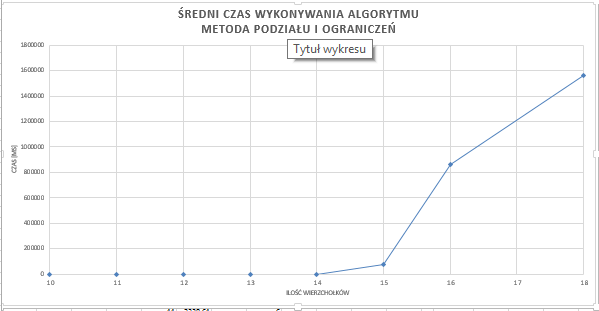
\includegraphics[width=0.7\linewidth]{bb}
		\end{center}
	
	
		
		
		\subsubsection{Czas działania algorytmu dla przeglądu zupełnego}
		\begin{table}[H]
			\centering
			\caption{Uśrednione wyniki dla 6 różnych ilości wierzchołków}
			\begin{tabular}{|c|c|}
				
				\hline Ilość miast  & czas działania algorytmu [ms] \\ 
				\hline 	6& 0,08 \\ 
				\hline  7& 0,5 \\ 
				\hline  8& 3,2\\ 
				\hline  9& 25,2\\ 
				\hline  10& 252,5\\ 
				\hline  11& 2340\\ 
				
				\hline 
			\end{tabular} 
		\end{table}
		Czas działania algorytmu dla przeglądu zupełnego ma charakter wykładniczy. Jest to metoda z najgorszą możliwą złożonością, jednakże z pewnością daje dobre wyniki.
		\begin{center}
			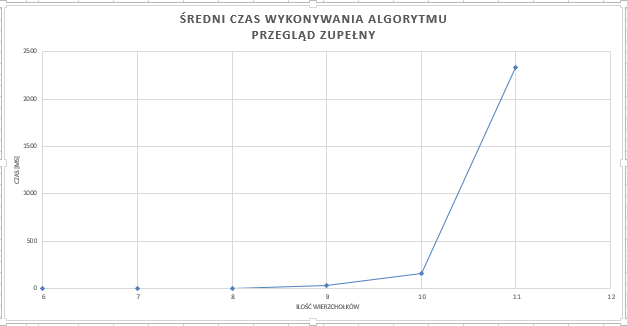
\includegraphics[width=0.7\linewidth]{bf}
		\end{center}
		\subsubsection{Porównanie czasów wykonywania algorytmu} 
		Wykres przedstawiony poniżej pozwala zaobserwować różnice pomiędzy czasem wykonywania algorytmu zarówno dla metody podziału i ograniczeń jak i przeglądu zupełnego. Nie jest zaskoczeniem, że czas sprawdzenia wszystkich możliwości jest dużo większy niż algorytm wykluczający pewne rozwiązania ze zbioru możliwych permutacji. 
		\begin{center}
			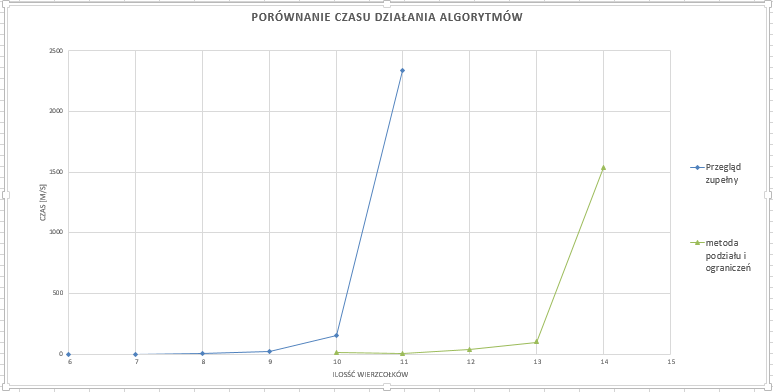
\includegraphics[width=0.7\linewidth]{bbVSbf.png}
		\end{center}
	
	\subsection{Analiza i ocena jakości}
\section{Podsumowanie}


\end{document}\documentclass{article}
